\chapter{Conclusion}

This project successfully addressed the precise AI planning and control problem - putting a shoelace on a shoe using bimanual robot, YuMi, and an external camera. All the specified requirements were met.

\begin{figure}[H]
\centering
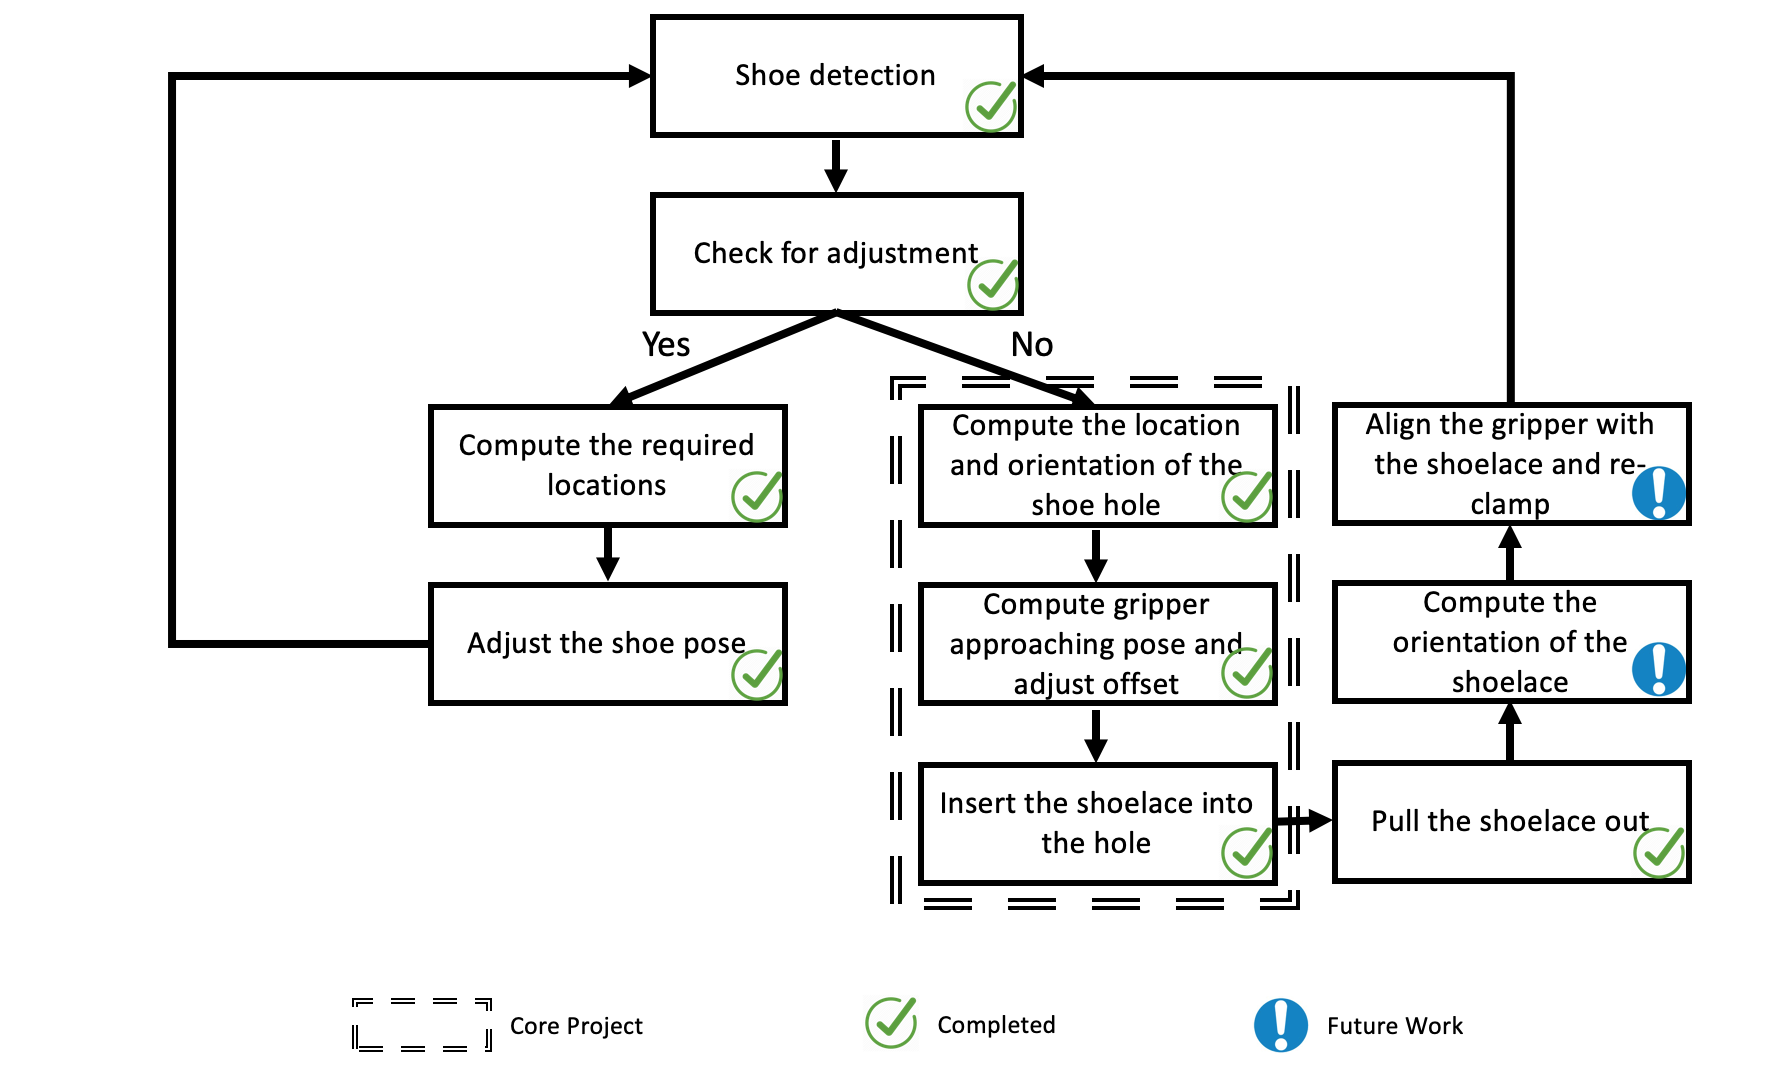
\includegraphics[width = \columnwidth]{conclusion/workflowcon.png}
\caption{The project achievements}
\label{workflowcon}
\end{figure}

Recall the system workflow, as shown in Figure \ref{workflowcon}, the core project which is passing the shoelace into a hole (with $4mm$ radius) has been successfully completed. Besides, YuMi equips with capabilities to adjust the pose of the shoe if necessary, as well as grab and pull the shoelace out to proper location for further manipulation after insertion. The corresponding success rates can be found in Table \ref{sris}.

\begin{table}[H]
\centering
\begin{tabular}{||c|c|c|c||}
\hline
Detection & Adjustment & Insertion & Pulling \\ \hline\hline
100\% & 95\% & 87\% & 91\% \\ \hline
\end{tabular}
\caption{The success rate of integrated system}
\label{sris}
\end{table}

For computer vision part, the two cameras, ASUS Xtion and ZED Mini, were correctly set up and calibrated. All computer vision algorithms in this project were implemented for both of them. As discussed in Section \ref{shoedetection}, the shoe can be successfully detected by employing YOLO, regardless of whether there are other interfering objects on the workbench. The calculation of required locations for shoe pose adjustment is introduced in Section \ref{shoeadjust}. All location conversions between camera frame and YuMi frame in this project are based on ROS $TF$ topic. Real-time 6D pose (3D location and 3D orientation) of shoe hole can also be estimated with high precision. The location is calculated based on some image processing techniques including color detection, blurred filters etc, details can be found in Section \ref{3dlocationestimation}. Moreover, I extracted the region of shoe and carefully set the color thresholds in advance to further reducing the impact of lighting conditions on the results. The method to compute accurate orientation of the shoe hole is mentioned in Section \ref{3DOrientationofShoeHole}, which is based on RANSAC. The orientation had great volatility, especially when using the low-resolution camera such as ASUS Xtion. Therefore, I introduced some pre-defined constraints to tackle this issue and finally averaged out the valid readings within a certain time.

For motion planning part, my algorithms can successfully plan and move YuMi for shoe and shoelace manipulation while avoiding potential collisions with the environments. The important details about interface and planning scene setup are told in Section \ref{motionplansetup}. The movement control, and related implementation methods such as setting joint goals and pose goals are discussed in Section \ref{movementcontrol}. The three safety poses throughout manipulation process are defined in Section \ref{safetyposescalculation}. Detailed shoe pose adjustment plan, shoelace insertion plan, shoelace grabbing plan and a series of their movement photo examples can be found in Section \ref{adj}, \ref{approachposegripper}, and \ref{shoelacegrabbing} respectively. Each plan contains several preparation postures and retreat postures. Both single-arm motion planning and dual-arm coordination are implemented. The accurate offset adjustment approach is in Section \ref{offsetadjustment}.

The advantages of the final integrated system are fast, relatively stable, and only require one camera. The qualitative and quantitative results can be found in Testing and Results Chapter. However, for my approach, the precision of 6D pose of shoe hole largely depends on the resolution of the camera. In addition, the offset needs to be adjusted every time the relative pose between the camera and the robot changes. These issues can be resolved by using the YuMi gripper camera, however it is currently unavailable. An alternative is to find an appropriate way to attach another small camera to YuMi's arm. By doing this, YuMi can adjust its gripper pose referenced to the pose of interested shoe hole continuously through the image feedback from the wrist camera. The accuracy is considered to be improved while the operation will become slower. More details are included in Section \ref{futurecamera}.


%A series of experiments have validated the proposed method, highlighting its strengths and drawbacks, but ultimately demonstrating high performance and versatility. The learning method was heavily inspired by combinations of previous works, but also introduced some novel techniques which contributed to the overall robustness of the system.

To complete the project extension, the last two parts in Figure \ref{workflowcon} workflow: "compute the orientation of the shoelace" and "align the gripper with the shoelace and reclamp" have to be implemented. The methods are no different from what have been described in the report. The former can be achieved by using color detection and RANSAC. Similarly, YuMi can align its right gripper with the colored head of shoelace and accomplish reclamping according to the approaches introduced in Section \ref{approachposegripper}. Adjusting shoe pose using single arm can refer to Section \ref{adj}. After that, the whole workflow is completed and the shoelace can be passed into every hole of the shoe.

Finally, there are some initial definitions for this project, such as the shoe and shoelace are marked, the shoelace is held by YuMi before insertion etc. Discussion about how to completely solve the problem of putting normal shoelace on a regular shoe can be found in the next chapter. 


%critical evaluation compare to previous ....product, algorithm, ...
 %- design choice 
 %- what did I learn
%advantages (positively and worthwhile) achievement!!
